\chapter{Teil1}
\label{cha:Teil1}

\begin{normalsize}
\begin{LARGE}

\section{Motivation}
\label{sec:Motivation}

Die Bereitstellung von Wärme und elektrischer Energie beeinflusst immer stärker das Klima. Nach wie vor wird zumeist die Energie fossiler Energieträger genutzt, um den Bedarf zu decken. Um den Einfluss unseres Energiebedarfs auf das Klima zu reduzieren, wurden in den vergangenen Jahrzehnten verschiedene Versuche unternommen die Energiebereitstellung auf nachhaltige Quellen umzustellen. In diesem Zusammenhang ergibt sich das Ziel die Anreicherung von in der Erde gespeichertem Kohlenstoff als Kohlenstoffdioxid oder in Form anderer klimabeeinflussender Gase, wie zum Beispiel Methan, in der Atmosphäre zu verhindern. 
Die am meisten genutzten Energiequellen sind hierbei die Wasserkraft, Wind und Sonne. Wobei die Nutzbarkeit aller drei genannten Energiequellen stark von den geologischen, klimatischen und geographischen Bedingungen der jeweiligen Region abhängt und in den meisten Regionen starken Leistungsschwankungen unterliegt, sodass sich Problematiken in der Speicherung der Energie ergeben. Außerdem werden in den nächsten Jahren die Endenergiepreise voraussichtlich steigen, da zum einen eine Verknappung der fossilen Brennstoffe auf lange Sicht unausweichlich ist und zum anderen die Umstellung auf regenerative Energien mit einem erheblichen Kostenaufwand verbunden ist.  Deshalb haben in den letzten Jahren die Bemühungen der Politik und verschiedener Marktteilnehmer zugenommen den Energieverbrauch zu senken. Für Privat genutzte Häuser und Wohnungen geschieht das in Deutschland vor allem über die "Verordnung über energiesparenden Wärmeschutz und energiesparende Analgentechnik bei Gebäuden", kurz EnEV \cite{.28.10.2015},  von staatlicher Seite. % [11]
Ziel der EnEV ist es durch eine gute Isolierung den Wärmeverlust der Häuser zu reduzieren. Um entsprechende Gebäude mit ausreichend Frischluft zu versorgen, wird die Luft mittels eines Lüftungssystems ausgetauscht. Durch den Einsatz von Wärmeübertragern wird der Wärmeverlust über die ausgetauschte Luft reduziert. 

Eine Konsequenz dieses Vorgehens in gemäßigten und kalten Klimaregionen ist ein Austrocknen der Raumluft. Die kalte Außenluft weist einen geringen absoluten Wassergehalt auf. Beim Erhitzen im Wärmeübertrager stellt sich so eine sehr geringe relative Feuchte ein. 
Da an Wohngebäude und Bürogebäude oft hohe Anforderungen bezüglich der Luftqualität gestellt werden, ist es in vielen Fällen sinnvoll die Luft auf eine Feuchtegehalt zu konditionieren, der von den Menschen als angenehm empfunden wird und keine negativen Auswirkungen auf ihren Gesundheitszustand oder ihre Leistungsfähigkeit hat. Eine detaillierte Zusammenfassung über die Auswirkungen zu trockener Luft liefert.\cite{JurgenSchniedersDr.RainerPflugerDr.WolfgangFeist.Oktober}
%Quelle einfügen Energetische Bewertung von Wohnungslüftungsgeräten mit Feuchterückgewinnung (12)
In feucht warmen Klimazonen tritt oft ein gegenteiliger Effekt auf. Die feucht warme Zuluft wird abgekühlt und gewinnt so an relativer Feuchte. Dies kann dazu führen, dass Feuchteschäden an Bauteilen oder am Interieur des Gebäudes entstehen oder es zur Bildung von Schimmel kommt. Entsprechend ist in vielen Fällen eine Trocknung der zugeführten Luft notwendig. \cite{Zhang.2010}
%[Zhang HB and Hiroshi Y. Analysis of indoor humidity environment in Chinese residential buildings. Build Environ 2010; 45(10): 2132–2140]
In Sonderfällen ist es möglich, dass bestimmte Raumklimabedingungen eingehalten werden müssen. Zum Beispiel erfordern bestimmte Lagerbedingungen oder Rahmenbedingungen für Produktionsabläufe oder Forschungsprozesse ein definiertes Raumklima. 
Das Trocknen beziehungsweise Befeuchten der Luft kostet viel Energie. Bei einem Luftbefeuchter muss hierzu die Verdampfungsenthalpie des Wassers überwunden werden. Eine Beschreibung des Energieverbrauchs von klassisch zur Trocknung von Luft eingesetzten Sorptionstrocknern findet sich beispielsweise in \cite{Zhang.2006}
% evtl Bild für Luftbefeuchter und Sorptionstrockner
Enthalpietauscher stellen eine Möglichkeit da, diese Energieaufwände zu reduzieren. 

\section{Enthalpieübertrager}
\label{Enthalpieübertrager}

Aus dem Stand der Technik sind vor allem Speicherenthalpieübertrager und membranbasierte Enthalpieübertrager bekannt. Beide Systeme übertragen neben Wärme auch Feuchte von einem feuchten auf einen trockenen Luftstrom. Die Triebkraft in beiden Systemen ist die Differenz des chemischen Potenzials, die ausgeglichen wird. 

\begin{figure} [h]
	%\centering
	\subfigure[Rotationsenthalpieübertrager]{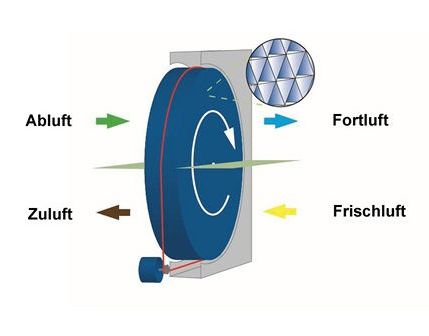
\includegraphics[width=0.49\textwidth]{Pictures/Rotation.jpg}}
	\subfigure[Membranbasierter Enthalpieübertrager]{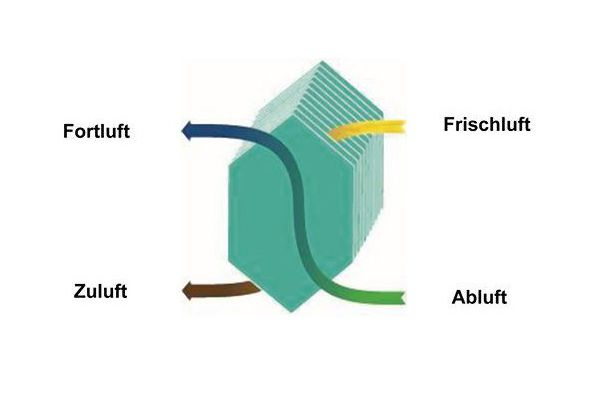
\includegraphics[width=0.49\textwidth]{Pictures/Enthalpieuebertrager.jpg}}
	\caption{Verschieden Ausführungsformen von Enthalpieübertragern}
	\label{fig:Enthalpieübertrager}
	
\end{figure}


Die Verbreitesten Speicherübertrager sind Rotationsübertrager. Rotationsübertrager weisen einen rotierende thermische Masse auf, die sich jeweils mit einem Teil der Masse im Zuluftstrom und mit einem anderen Teil der Masse im Abluftstrom befindet. Durch die Rotation kann die Masse thermische Energie in einem Luftstrom aufnehmen und nach dem Weiterrotieren im anderen Luftstrom abgeben. Analog funktioniert die Übertragung der Feuchte, wobei die Feuchte entweder von einem Sorptionsmaterial aufgenommen und wieder abgegeben wird oder in einem Luftstrom an der Masse kondensiert und im anderen Luftstrom wieder verdampft. Rotationsübertrager befinden sich bereits seit einigen Jahren kommerziell im Einsatz und wurden bereits entsprechend detailliert untersucht. Ein detailliertes Modell von Rotationsübertagern liefert eine Untersuchng von Zhang\cite{Zhang.2002}. Die Artikel \cite{Zhang.2006} und \cite{JustoAlonso.2015} vergleichen unterschiedliche Optionen der Lufttrocknung.
Membranbasierte Enthalpieübertrager sind erst seit wenigen Jahren kommerziell im Einsatz, sodass es bisher nur wenige Untersuchungen zu ihnen existieren. Die Wärme wird dann über die Membran von einem Luftstrom über an den anderen übertragen. Analog zum übertragenen Wärmestrom wird die Feuchte übertragen, das heißt Wasser wird vom Membranmaterial absorbiert, diffundiert durch die Membran und desorbiert auf der anderen Seite in den Luftstrom. Die Geometrien, die dabei für den Enthalpieübertrager verwendet werden, entsprechen denen, die bei klassischen Wärmeübertragern zum Einsatz kommen. In kommerziellen Anwendungen kommen Kreuzstromübertrager und Kreuzgegenstromübertrager zur Anwendung, wobei auch Gegenstromübertrager und "hollow fibre" Module mögliche Bauform darstellen. Kreuzstromübertrager sind im Vergleich zu Gegenstromübertragern Kostengünstig herstellbar und benötigen nur geringen Bauraum, daher sind sie die bisher häufigste Bauform bei Enthalpietauschern. Gegenstromübertrager haben im Gegensatz dazu einen hohen Wirkungsgrad. Deshalb hält vor allem eine Mischform aus beidem, der Kreuzgegenstromübertrager, immer stärker Einzug in die kommerzielle Nutzung. Hollow fibre Module ermöglichen hohe Übertragungsflächen bei kleinem Bauraum und somit hohe Übertragungsraten für Wärme und Feuchte. Dies erläutern auch die Artikel von Zhang und Bui \cite{Zhang.2010} \cite{Bui.2010}. Nachteilig ist jedoch ein sehr hoher Druckverlust in den Modulen, der bisher verhindert hat, das diese Bauform sich in kommerziellen Anwendungen durchsetzen konnte. 

\begin{figure} [h]
	\centering
	%\includegraphics[width=400]{pictures/Vergleich_Geometirie.jpg}
	%\caption{Geometrien}
	%\label{fig:verschiendene Enthalpieübertrager-Geometrien}
	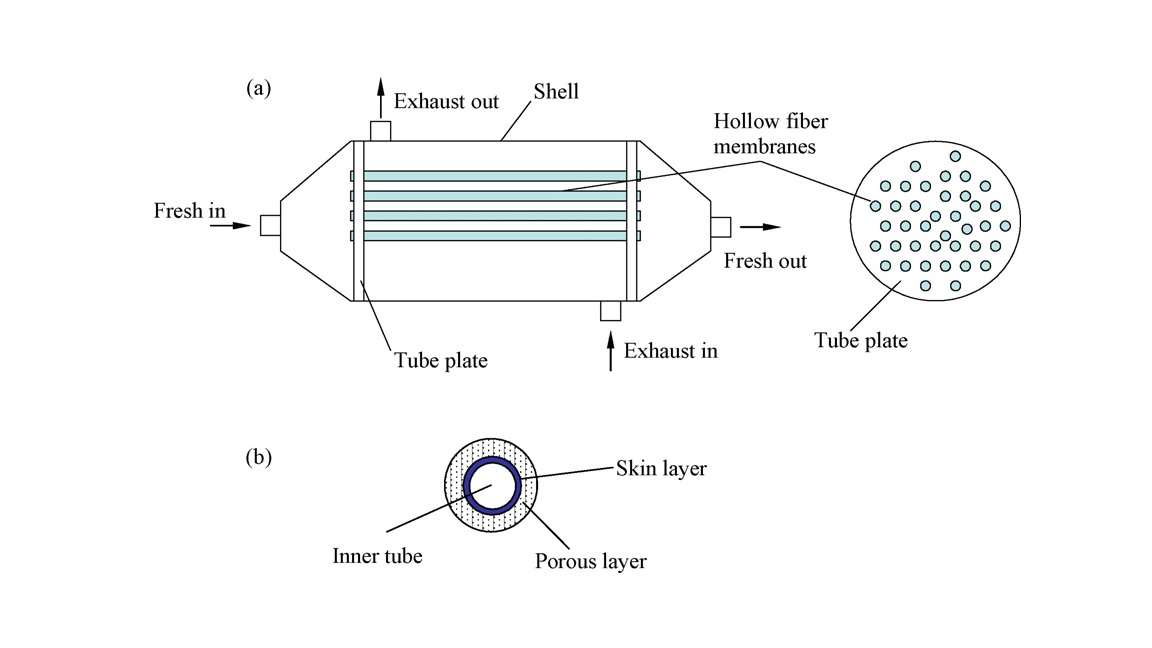
\includegraphics[width=0.98\textwidth]{pictures/hollow_fibre.jpg}
	\caption{hollow fibre}
	\label{fig:hollow fibre Modul}
\end{figure}

Ein Vergleich zwischen Rotationsübertragern und membranbasierten Enthalpietauschern fällt je nach Untersuchung unterschiedlich aus. Grundlegend haben jedoch membranbasierte Enthalpietauscher den Vorteil, dass sie keine beweglichen (rotierenden) Komponenten haben, was sie weniger verschleißanfällig macht und die Geräuschemissionen senkt. Außerdem muss keine Energie zum Antrieb eines Rotors aufgewendet werden. In den meisten Fällen besitzen membranbasierte Enthalpieübertrager den höheren Wirkungsgrad. \cite{JustoAlonso.2015}  %weitere Quelle
Nachteilig ist, dass Enthalpieübertrager nicht regelbar sind. Laut % Quelle
ist es bei besonders feucht-warmen Tagen daher möglich, dass ein Enthalpieübertrager zur Feuchterückgewinnung der Zuluft zu viel Wasser zuführt. Dies könnte nur durch einen Bypass, eine Trockner oder einen Austausch des Enthalpieübertragers durch einen Wärmeübertrager für die entsprechende Jahreszeit verhindert werden. Außerdem können die membranbasierten Übertrager bei zu kalten Temperaturen zufrieren und müssen daher in einigen Klimazonen mit Vorheizern ausgestattet werden. Derzeit beherrschen Rotationsübertrager vor allem den Markt bei großen Anwendungsfällen während Enthalpieübertrager vor allem für Wohnungs- und Einzelraumlüftungen genutzt werden.  


\section{Membran}

Membranen lassen sich in dichte und poröse Membranen unterteilen. Poröse Membranen weisen Poren auf, die größer sind als die Partikel, die durch die Membran übertragen werden. Daher findet der Stofftransport aufgrund von.... statt. Dichte Membranen weisen hingegen keine oder nur sehr kleine Poren auf.  Der Stofftransport findet bei dichten Membranen auf Grund von Diffusionsprozessen statt. % evtl. noch sorption erwähnen
Dies führt in den meisten Fällen zu einer deutlich erhöhten Selektivität und einer geringeren Permeabilität im Vergleich zu porösen Membranen. Da im vorliegenden Anwendungsfall Wasserdampf als Permeat die Membran passieren soll und kleine gasförmige Moleküle der Luft, wie Stickstoff zurückgehalten werden sollen, ist eine Dichte Membran sinnvoll, da nur so eine ausreichende Selektivität gegenüber den gasförmigen Komponenten gewährleistet werden kann. Um dennoch eine möglichst hohe Permeabilität gegenüber Wasserdampf zu gewährleisten ist es zielführend eine möglichst dünne Membran zu verwenden. Um die dünnen dichten Membranen mechanische zu stabilisieren wird die dichte Membran in einigen Fällen durch eine poröse Membran gestützt. Die poröse Membran hat kaum negative Auswirkungen auf die Permeabilität, da die Transportgeschwindigkeiten in porösen Membranen wesentlichen höher sind als in dichten Membranen. Gleichzeitig ist jedoch anzunehmen, dass Spacermaterialien und porösen Membranen Einfluss auf die Strömung nehmen und somit auf die Wärmeübergangskoeffizienten und Sorptionseigenschaften an der Membranoberfläche. %auf wasseraffinität eingehen

\begin{figure} [h]
	\centering
	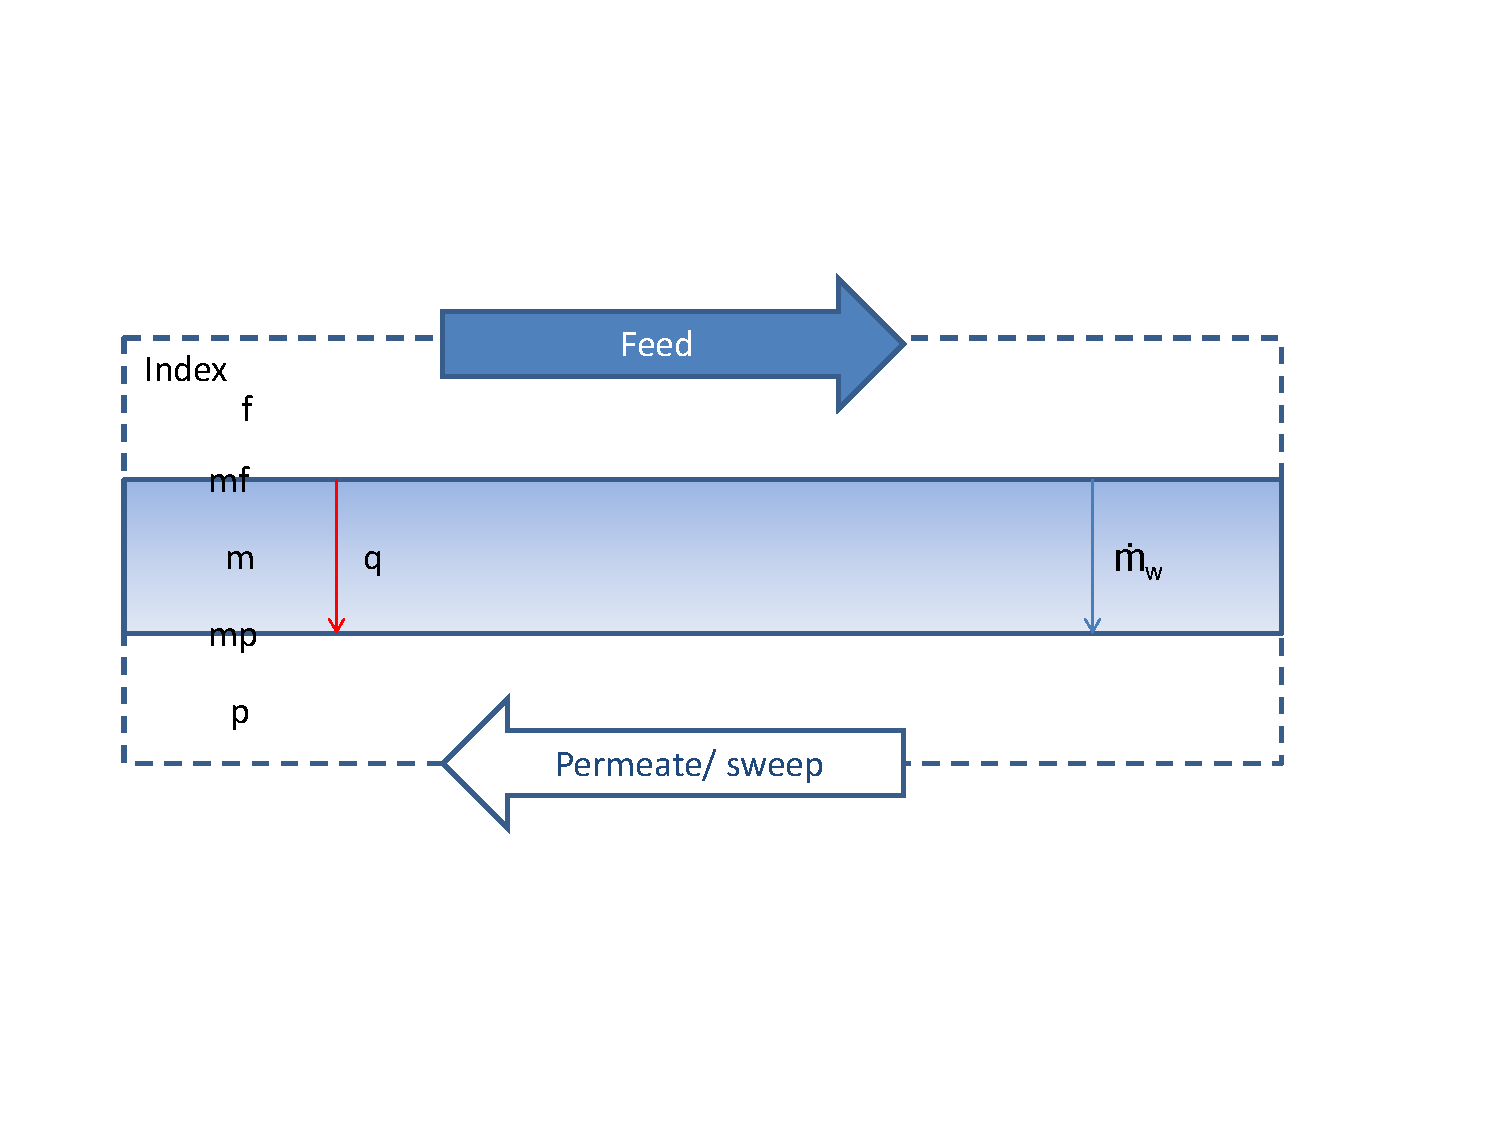
\includegraphics[width=0.98\textwidth]{pictures/Membran.pdf}
	\caption{Membran}
	\label{Membran}
\end{figure}

In Enthalpieübertragern werden derzeit Membranen aus Papier oder Polymeren eingesetzt. Die technische Weiterentwicklung der Polymermembranen über die letzten Jahre hat dazu geführt, das mittlerweile fast ausschließlich Polymermembranen zu Einsatz kommen, da diese deutlich höhere Permeabilitäten aufweisen. 

%Der Transport des Wasser von einem Luftstrom in den anderen Luftstrom durch die Membran lässt sich in 3 Phasen einteilen. Zuerst wird das Wasser auf einer Seite von der Membran Absorbiert, dann diffundiert das flüssige Wasser durch die Membran und wird auf der anderen Seite der Membran desobiert und an den Luftstrom abgegeben. 

% bild zum Transportprozess



Ein klassischer Vergleich über Wirkungsgrade, ist nur bedingt Sinnvoll. Die dabei bisher verwendeten Wirkungsgrade sind der Wärmeübertragungsgrad $\eta_{t}$ und der Enthalpiewirkungsgrad $\eta_{h}$. Der Wärmeübertragungsgrad hängt dabei rein von der thermischen Energie ab, 
%\begin{equation}

%\end{equation}.

Der Enthalpiewirkungsgrad beschreibt die gesamte übertragene Energie, also inklusive der Enthalpie die im übertragenen Wasserdampf steckt,
%\begin{equation}

%\end{equation}

Der Wärmeübertragungsgrad bei einem reine Wärmeübertrager ist fast immer größer, als bei einem Enthalipeübertrager und andersherum weißt der Enthalpieübertrager einen größeren gesamten Enthalpiewirkungsgrad auf.  Da membranbasierte Enthalpieübertrager ungeregelt Feuchte in den Zuluftstrom übertragen, ist die eine Bewertung anhand der Gesamtenthalpie oft nicht gerechtfertigt, da teilweise mehr feuchte übertragen wird als benötigt. %evtl. noch auf Normzustand und Abweichung über das Jahr eingehen
Der Wärmeübertragungsgrad stellt kein geeignetes Vergleichskriterium dar, da die übertragene Feuchte nicht berücksichtigt wird, die eine Hauptfunktion des Enthalpietauschers darstellt.




In dieser Arbeit sollen insbesondere membranbasierte Enthalpietauscher untersucht werden und Vergleichsgrößen die gefunden werden, die eine Energierückgewinnung mittels Enthalpietauschern mit anderen Systemen vergleichbar machen. Des Weiteren soll ein Modell der Enthalpieübertrager angefertigt werden, das zukünftig als Grundlage für Simulationen und für eine Weiterentwicklung der Modelle dienen soll, um Enthalpieübertrager auch in größeren Systemen simulativ einbinden zu können.  


\section{Stand der Technik}

Bisherige Veröffentlichungen zu Untersuchungen beschreiben vor allem Kennzahlermittlungen und die Genauigkeit bestimmter Modell-Ansätze. Für einen Überblick über die Veröffentlichungslage und den derzeitigen Stand der Technik empfehlen sich vor allem die Artikel....
Als Modelle werden vor allem Lösungs-Diffusions-Modelle vorgeschlagen. Sie beruhen auf der Annahme, dass Wasserdampf an der Oberfläche der Membran absorbiert wird, durch die Membran diffundiert und auf der gegenüberliegende Seite wieder an die Luft abgegeben wird. Aus dieser Betrachtungsweise ergeben sich verschiedene Möglichkeiten das System zu beschreiben. 
Grundsätzlich lassen sich die Publikationen in Bewertungs- beziehungsweise Komponentenoptimierungsorientierte und Modellermittelnde Untersuchungen unterteilen. Die bewertungsorientierten Arbeiten nutzen für den Vergleich verschiedener Bauweisen, Geometrien und Prinzipien vor bekannte Bewertungsgrößen wie die den Wärmeübertragungsgrad, die Feuchteübertragungsgrad oder den totalen Enthalpieübertragungsgrad. Sowie die Number of transfer units.
Bisherige Untersuchungen zur Modellbildung beziehen sich weitestgehend auf die Bestimmung Grundlegender Kenngrößen oder Beschreibungswerte die Analog zu bekannten Systemen definiert wurden. Hierbei kommen vor allem Größen zum Einsatz, die die unterschiedlichen für sich einzeln bereits bekannten Teilbereich der ablaufenden Prozesse in Beziehung zueinander setzt. So lassen sich  die Strömungseigenschaften, die Wärmeübertragung und die Feuchteübertragung getrennt voneinander betrachten und mit Kennzahlen, die ggf. von gewissen Parametern abhängen miteinander verknüpfen. Außerdem wurden in verschiedenen Artikeln unterschiedliche Annahmen überprüft beziehungsweise ihre Gültigkeit validiert. 

In dieser Arbeit soll im Gegensatz dazu ein Modell eines ermittelt werden das einen kommerziell einsatzfähigen Enthalpieübertrager beschreibt. Dabei liegt der Schwerpunkt nicht auf der Ermittlung der physikalischen Grundwerte oder Gültigkeit der physikalischen Modelle  und der zu Grunde liegenden Annahmen sondern auf der Beschreibung des Verhaltens des praktische eingesetzten Systems unter bestimmten Umgebungsbedingungen und in bestimmten Anwendungsfällen. Der Schwerpunkt liegt hier wiederum auf dem deutschen Klimaraum und dem Einsatz in Wohnraumlüftungen. 
%Die Betrachtungsweise bleibt also empirischer und und beschäftigt sich nicht mit den Materialeigenschaften
Ziel ist eine Modell zu generieren das Abhängig von Anforderungsprofilen und Umgebungsbedingungen eine Bewertung der Enthalpieübertragern insbesondere im Vergleich zu alternativen Systemen, wie z.B. Speicherenthalieübertragern und klassischen Wärmeübertragern mit entsprechender Lufttrocknung. Zu diesem Zweck sollen auch Bewertungsgrößen definiert werden die eine sinnvollen Vergleich der verschiedenen Größen zulassen. 




Enthalpieübertrager
Ein membranbasierter Enthalpietauscher nutzt die selektiven Eigenschaften einer Membran um einen Konzentrationsausgleich an Wasser zwischen den beiden Luftströmen auszugleichen. Dabei werden ansonsten die Funktionsweisen und Geometrien von klassischen Wärmeübertragern genutzt. Entsprechend lassen sich Kreuz-, Gegenstrom, Kreuz-Gegenstrom- und Gleichstrom Geometrien realisieren. Wobei die Kreuzstromgeometrie die am weitesten Verbreitete Geometrie ist, da sie die einfachste und kostengünstigste Version darstellt. Mit der Gegenstromgeometrie lässt sich der höchste Wirkungsgrad erreichen. Deshalb kommt auch diese Geometrie, sowie die Kreuz-Gegenstromgeometrie, als Kompromiss zwischen Gegenstrom- und Kreuzstromgeometrie, zum Einsatz. 
Ein weitere Unterscheidungskriterien sind der Anwendungsbereich, die Richtung des Feuchtetransports, die verwendete Membran,

Klassischer Anwenungsbereicht dieser Enthalpietauscher ist bisher die Einzelraumlüftung für Wohnungen und Büroräume. Aber auch größere Anwendungen sind mittlerweile möglich. Bisher liefern viele Anbieter die Lüftungsgeräte mit der Option aus den Enthalpietauscher im Sommer gegen einen Wärmeübertrager zu tauschen. Dies isst der Problematik geschuldet, dass die Enthalpieübertreager im Gegensatz zu den Rotationsübertragern nicht regelbar sind. Es besteht die Befürchtung, dass die im Sommer, wenn die Luftfeuchtigkeit in der Zuluft ohnehin hoch ist, eine weitere ungeregelte Anfeuchtung zu Schimmelbildung und Feuchteschäden führen kann. Hierzu gibt es in der Literatur verschiedene Ansichten. ...









Membranen sind bereits seit langem bekannt und kommen in technischen Bereichen bereits in vielen Gebieten zur Anwendung. Dabei unterliegen die ablaufenden Prozesse und Trennverfahren unterschiedlichen physikalischen Ursachen. In Enthalpieübertragern wird eine hohe Permeabilität der Membran gegenüber Wasser gefordert und eine geringe Permeabilität gegenüber verschiedene Gase, wie zum Beispiel Kohlenstoffdioxid und Stickstoff. Entsprechend werden in dieser Arbeit auch nur Membranen und Ihre physikalischen Grundlagen behandelt, die diese Eigenschaften erfüllen. Um eine ausreichende Isolierung gegen Gase zu erhalten ist es sinnvoll dichte Membranen zu nutzen. Naheliegend sind Membranen, die auf osmotischen Prinzipien beruhen. Osmotische Membranen werden bisher vor allem eingesetzt, um Wasser zu reinigen. 

 
\end{LARGE}
\end{normalsize}


\begin{table}[htb]
\centering
\caption{Das ist eine Testtabelle}\vspace{6pt}
\label{fig:PCM_Slurry1}
\begin{tabular}{cr} 
\hline
\textbf{Überschrift links} & \textbf{Überschrift rechts}\\
\hline 
links oben & rechts oben \\  
links unten & rechts unten \\ 
\hline 
\end{tabular}
\label{tab:Tabelle}
\end{table}

